\documentclass[12 pt]{article}
\usepackage[a4paper,top=3.5cm,bottom=3cm,left=3cm,right=3cm]{geometry}
\usepackage{graphicx} 
\usepackage{amssymb}
\usepackage{lmodern}
\usepackage{setspace}
\author{Vanessa Braglia}
\title{The swiss scientific social network}
\date{\today}

\onehalfspacing

\begin{document}
\fontfamily{lmr}\selectfont
\maketitle 
\newpage
\tableofcontents
\newpage
\section{Introduction}
A social network consists of a set of objects connected to each other by social relations. The best way to model social networks is using graphs (see an example in Figure 1): the objects (entities) are represented as nodes and the connections as edges between two different nodes. \\
\begin{figure} [h!]
\centering 
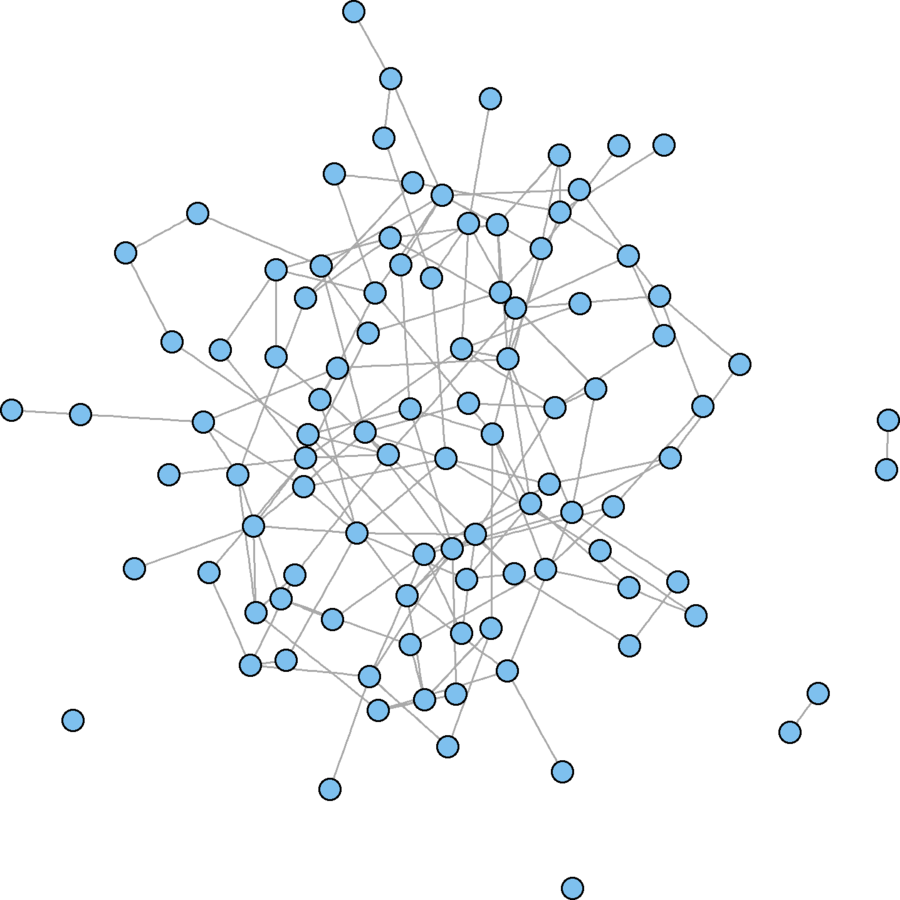
\includegraphics[scale=0.5]{graph.png}
\caption{Example of social network graph}
\end{figure}
\\
The goal of this project is to create a social network of the computational science authors belonging to Swiss institutions and then analyze the relative graph.\\
The first step will be retrieving the information necessary for the construction of the social network based on coauthorship relations; then I will implement and apply the PR algorithm for the analysis of the graph.
The results will provide an interesting picture of the different research scenarios in Switzerland and how they interact with each other.
The most common example we can take is the World Wide Web (WWW) where we have web pages as nodes connected by hyperlinks, the edges. In order to rank the huge amount of web pages and optimize the search for a particular page, more then twenty years ago was developed the PageRank (PR) algorithm. PageRank works on the graph representing the WWW, so it is applicable to all graphs representing social network.

The goal of this project is to create a social network of the scientific authors belonging to Swiss institutions, then analyze the relative graph and apply the PR algorithm.\\
The first step will be retrieving the information necessary for the construction of the social network based on coauthorship relations; then I will implement and apply the PR algorithm for the analysis of the graph.
The results will provide an interesting picture of the different research scenarios in Switzerland and how they interact with each other.
\end{document}
